
%% bare_conf.tex
%% V1.3
%% 2007/01/11
%% by Michael Shell
%% See:
%% http://www.michaelshell.org/
%% for current contact information.
%%
%% This is a skeleton file demonstrating the use of IEEEtran.cls
%% (requires IEEEtran.cls version 1.7 or later) with an IEEE conference paper.
%%
%% Support sites:
%% http://www.michaelshell.org/tex/ieeetran/
%% http://www.ctan.org/tex-archive/macros/latex/contrib/IEEEtran/
%% and
%% http://www.ieee.org/

%%*************************************************************************
%% Legal Notice:
%% This code is offered as-is without any warranty either expressed or
%% implied; without even the implied warranty of MERCHANTABILITY or
%% FITNESS FOR A PARTICULAR PURPOSE! 
%% User assumes all risk.
%% In no event shall IEEE or any contributor to this code be liable for
%% any damages or losses, including, but not limited to, incidental,
%% consequential, or any other damages, resulting from the use or misuse
%% of any information contained here.
%%
%% All comments are the opinions of their respective authors and are not
%% necessarily endorsed by the IEEE.
%%
%% This work is distributed under the LaTeX Project Public License (LPPL)
%% ( http://www.latex-project.org/ ) version 1.3, and may be freely used,
%% distributed and modified. A copy of the LPPL, version 1.3, is included
%% in the base LaTeX documentation of all distributions of LaTeX released
%% 2003/12/01 or later.
%% Retain all contribution notices and credits.
%% ** Modified files should be clearly indicated as such, including  **
%% ** renaming them and changing author support contact information. **
%%
%% File list of work: IEEEtran.cls, IEEEtran_HOWTO.pdf, bare_adv.tex,
%%                    bare_conf.tex, bare_jrnl.tex, bare_jrnl_compsoc.tex
%%*************************************************************************

% *** Authors should verify (and, if needed, correct) their LaTeX system  ***
% *** with the testflow diagnostic prior to trusting their LaTeX platform ***
% *** with production work. IEEE's font choices can trigger bugs that do  ***
% *** not appear when using other class files.                            ***
% The testflow support page is at:
% http://www.michaelshell.org/tex/testflow/



% Note that the a4paper option is mainly intended so that authors in
% countries using A4 can easily print to A4 and see how their papers will
% look in print - the typesetting of the document will not typically be
% affected with changes in paper size (but the bottom and side margins will).
% Use the testflow package mentioned above to verify correct handling of
% both paper sizes by the user's LaTeX system.
%
% Also note that the "draftcls" or "draftclsnofoot", not "draft", option
% should be used if it is desired that the figures are to be displayed in
% draft mode.
%
\documentclass[a4paper,conference]{IEEEtran}
% Add the compsoc option for Computer Society conferences.
%
% If IEEEtran.cls has not been installed into the LaTeX system files,
% manually specify the path to it like:
% \documentclass[conference]{../sty/IEEEtran}





% Some very useful LaTeX packages include:
% (uncomment the ones you want to load)


% *** MISC UTILITY PACKAGES ***
%
%\usepackage{ifpdf}
% Heiko Oberdiek's ifpdf.sty is very useful if you need conditional
% compilation based on whether the output is pdf or dvi.
% usage:
% \ifpdf
%   % pdf code
% \else
%   % dvi code
% \fi
% The latest version of ifpdf.sty can be obtained from:
% http://www.ctan.org/tex-archive/macros/latex/contrib/oberdiek/
% Also, note that IEEEtran.cls V1.7 and later provides a builtin
% \ifCLASSINFOpdf conditional that works the same way.
% When switching from latex to pdflatex and vice-versa, the compiler may
% have to be run twice to clear warning/error messages.






% *** CITATION PACKAGES ***
%
\usepackage{cite}
% cite.sty was written by Donald Arseneau
% V1.6 and later of IEEEtran pre-defines the format of the cite.sty package
% \cite{} output to follow that of IEEE. Loading the cite package will
% result in citation numbers being automatically sorted and properly
% "compressed/ranged". e.g., [1], [9], [2], [7], [5], [6] without using
% cite.sty will become [1], [2], [5]--[7], [9] using cite.sty. cite.sty's
% \cite will automatically add leading space, if needed. Use cite.sty's
% noadjust option (cite.sty V3.8 and later) if you want to turn this off.
% cite.sty is already installed on most LaTeX systems. Be sure and use
% version 4.0 (2003-05-27) and later if using hyperref.sty. cite.sty does
% not currently provide for hyperlinked citations.
% The latest version can be obtained at:
% http://www.ctan.org/tex-archive/macros/latex/contrib/cite/
% The documentation is contained in the cite.sty file itself.


%% TILDES
\usepackage[utf8]{inputenc}
%\usepackage[spanish]{babel}

\renewcommand{\tablename}{Tabla}

% *** GRAPHICS RELATED PACKAGES ***
%

\ifCLASSINFOpdf
  \usepackage[pdftex]{graphicx}
  % declare the path(s) where your graphic files are
  \graphicspath{{./eps/} }%{../jpeg/}}
  % and their extensions so you won't have to specify these with
  % every instance of \includegraphics
  \DeclareGraphicsExtensions{.eps} %.pdf,.jpeg,.png}
\else
  % or other class option (dvipsone, dvipdf, if not using dvips). graphicx
  % will default to the driver specified in the system graphics.cfg if no
  % driver is specified.
  \usepackage[dvips]{graphicx}
  % declare the path(s) where your graphic files are
  \graphicspath{{./eps/}
  % and their extensions so you won't have to specify these with
  % every instance of \includegraphics
  \DeclareGraphicsExtensions{.eps}
\fi
% graphicx was written by David Carlisle and Sebastian Rahtz. It is
% required if you want graphics, photos, etc. graphicx.sty is already
% installed on most LaTeX systems. The latest version and documentation can
% be obtained at: 
% http://www.ctan.org/tex-archive/macros/latex/required/graphics/
% Another good source of documentation is "Using Imported Graphics in
% LaTeX2e" by Keith Reckdahl which can be found as epslatex.ps or
% epslatex.pdf at: http://www.ctan.org/tex-archive/info/
%
% latex, and pdflatex in dvi mode, support graphics in encapsulated
% postscript (.eps) format. pdflatex in pdf mode supports graphics
% in .pdf, .jpeg, .png and .mps (metapost) formats. Users should ensure
% that all non-photo figures use a vector format (.eps, .pdf, .mps) and
% not a bitmapped formats (.jpeg, .png). IEEE frowns on bitmapped formats
% which can result in "jaggedy"/blurry rendering of lines and letters as
% well as large increases in file sizes.
%
% You can find documentation about the pdfTeX application at:
% http://www.tug.org/applications/pdftex





% *** MATH PACKAGES ***
%
\usepackage[cmex10]{amsmath}
% A popular package from the American Mathematical Society that provides
% many useful and powerful commands for dealing with mathematics. If using
% it, be sure to load this package with the cmex10 option to ensure that
% only type 1 fonts will utilized at all point sizes. Without this option,
% it is possible that some math symbols, particularly those within
% footnotes, will be rendered in bitmap form which will result in a
% document that can not be IEEE Xplore compliant!
%
% Also, note that the amsmath package sets \interdisplaylinepenalty to 10000
% thus preventing page breaks from occurring within multiline equations. Use:
\interdisplaylinepenalty=2500
% after loading amsmath to restore such page breaks as IEEEtran.cls normally
% does. amsmath.sty is already installed on most LaTeX systems. The latest
% version and documentation can be obtained at:
% http://www.ctan.org/tex-archive/macros/latex/required/amslatex/math/





% *** SPECIALIZED LIST PACKAGES ***
%
%\usepackage{algorithmic}
% algorithmic.sty was written by Peter Williams and Rogerio Brito.
% This package provides an algorithmic environment fo describing algorithms.
% You can use the algorithmic environment in-text or within a figure
% environment to provide for a floating algorithm. Do NOT use the algorithm
% floating environment provided by algorithm.sty (by the same authors) or
% algorithm2e.sty (by Christophe Fiorio) as IEEE does not use dedicated
% algorithm float types and packages that provide these will not provide
% correct IEEE style captions. The latest version and documentation of
% algorithmic.sty can be obtained at:
% http://www.ctan.org/tex-archive/macros/latex/contrib/algorithms/
% There is also a support site at:
% http://algorithms.berlios.de/index.html
% Also of interest may be the (relatively newer and more customizable)
% algorithmicx.sty package by Szasz Janos:
% http://www.ctan.org/tex-archive/macros/latex/contrib/algorithmicx/




% *** ALIGNMENT PACKAGES ***
%
%\usepackage{array}
% Frank Mittelbach's and David Carlisle's array.sty patches and improves
% the standard LaTeX2e array and tabular environments to provide better
% appearance and additional user controls. As the default LaTeX2e table
% generation code is lacking to the point of almost being broken with
% respect to the quality of the end results, all users are strongly
% advised to use an enhanced (at the very least that provided by array.sty)
% set of table tools. array.sty is already installed on most systems. The
% latest version and documentation can be obtained at:
% http://www.ctan.org/tex-archive/macros/latex/required/tools/


%\usepackage{mdwmath}
%\usepackage{mdwtab}
% Also highly recommended is Mark Wooding's extremely powerful MDW tools,
% especially mdwmath.sty and mdwtab.sty which are used to format equations
% and tables, respectively. The MDWtools set is already installed on most
% LaTeX systems. The lastest version and documentation is available at:
% http://www.ctan.org/tex-archive/macros/latex/contrib/mdwtools/


% IEEEtran contains the IEEEeqnarray family of commands that can be used to
% generate multiline equations as well as matrices, tables, etc., of high
% quality.


%\usepackage{eqparbox}
% Also of notable interest is Scott Pakin's eqparbox package for creating
% (automatically sized) equal width boxes - aka "natural width parboxes".
% Available at:
% http://www.ctan.org/tex-archive/macros/latex/contrib/eqparbox/





% *** SUBFIGURE PACKAGES ***
%\usepackage[tight,footnotesize]{subfigure}
% subfigure.sty was written by Steven Douglas Cochran. This package makes it
% easy to put subfigures in your figures. e.g., "Figure 1a and 1b". For IEEE
% work, it is a good idea to load it with the tight package option to reduce
% the amount of white space around the subfigures. subfigure.sty is already
% installed on most LaTeX systems. The latest version and documentation can
% be obtained at:
% http://www.ctan.org/tex-archive/obsolete/macros/latex/contrib/subfigure/
% subfigure.sty has been superceeded by subfig.sty.



%\usepackage[caption=false]{caption}
%\usepackage[font=footnotesize]{subfig}
% subfig.sty, also written by Steven Douglas Cochran, is the modern
% replacement for subfigure.sty. However, subfig.sty requires and
% automatically loads Axel Sommerfeldt's caption.sty which will override
% IEEEtran.cls handling of captions and this will result in nonIEEE style
% figure/table captions. To prevent this problem, be sure and preload
% caption.sty with its "caption=false" package option. This is will preserve
% IEEEtran.cls handing of captions. Version 1.3 (2005/06/28) and later 
% (recommended due to many improvements over 1.2) of subfig.sty supports
% the caption=false option directly:
%\usepackage[caption=false,font=footnotesize]{subfig}
%
% The latest version and documentation can be obtained at:
% http://www.ctan.org/tex-archive/macros/latex/contrib/subfig/
% The latest version and documentation of caption.sty can be obtained at:
% http://www.ctan.org/tex-archive/macros/latex/contrib/caption/




% *** FLOAT PACKAGES ***
%
%\usepackage{fixltx2e}
% fixltx2e, the successor to the earlier fix2col.sty, was written by
% Frank Mittelbach and David Carlisle. This package corrects a few problems
% in the LaTeX2e kernel, the most notable of which is that in current
% LaTeX2e releases, the ordering of single and double column floats is not
% guaranteed to be preserved. Thus, an unpatched LaTeX2e can allow a
% single column figure to be placed prior to an earlier double column
% figure. The latest version and documentation can be found at:
% http://www.ctan.org/tex-archive/macros/latex/base/



%\usepackage{stfloats}
% stfloats.sty was written by Sigitas Tolusis. This package gives LaTeX2e
% the ability to do double column floats at the bottom of the page as well
% as the top. (e.g., "\begin{figure*}[!b]" is not normally possible in
% LaTeX2e). It also provides a command:
%\fnbelowfloat
% to enable the placement of footnotes below bottom floats (the standard
% LaTeX2e kernel puts them above bottom floats). This is an invasive package
% which rewrites many portions of the LaTeX2e float routines. It may not work
% with other packages that modify the LaTeX2e float routines. The latest
% version and documentation can be obtained at:
% http://www.ctan.org/tex-archive/macros/latex/contrib/sttools/
% Documentation is contained in the stfloats.sty comments as well as in the
% presfull.pdf file. Do not use the stfloats baselinefloat ability as IEEE
% does not allow \baselineskip to stretch. Authors submitting work to the
% IEEE should note that IEEE rarely uses double column equations and
% that authors should try to avoid such use. Do not be tempted to use the
% cuted.sty or midfloat.sty packages (also by Sigitas Tolusis) as IEEE does
% not format its papers in such ways.





% *** PDF, URL AND HYPERLINK PACKAGES ***
%
%\usepackage{url}
% url.sty was written by Donald Arseneau. It provides better support for
% handling and breaking URLs. url.sty is already installed on most LaTeX
% systems. The latest version can be obtained at:
% http://www.ctan.org/tex-archive/macros/latex/contrib/misc/
% Read the url.sty source comments for usage information. Basically,
% \url{my_url_here}.





% *** Do not adjust lengths that control margins, column widths, etc. ***
% *** Do not use packages that alter fonts (such as pslatex).         ***
% There should be no need to do such things with IEEEtran.cls V1.6 and later.
% (Unless specifically asked to do so by the journal or conference you plan
% to submit to, of course. )


% correct bad hyphenation here
\hyphenation{op-tical net-works semi-conduc-tor}


\begin{document}
%
% paper title
% can use linebreaks \\ within to get better formatting as desired
\title{ADC $\Sigma\Delta$ en FPGA}


% author names and affiliations
% use a multiple column layout for up to three different
% affiliations
\author{
\IEEEauthorblockN{Carducci, Nahuel \\ Demski, Andr\'es\\  Kukulanski, Ariel\\  Paunovic, Iv\'an }
\IEEEauthorblockA{Departamento de Ingenier\'ia Electr\'onica,\\Universidad Tecnol\'ogica Nacional, Facultad Regional Buenos Aires.}
}
%\and
%\IEEEauthorblockN{Homer Simpson}
%\IEEEauthorblockA{Twentieth Century Fox\\
%Springfield, USA\\
%Email: homer@thesimpsons.com}
%\and
%\IEEEauthorblockN{James Kirk\\ and Montgomery Scott}
%\IEEEauthorblockA{Starfleet Academy\\
%San Francisco, California 96678-2391\\
%Telephone: (800) 555--1212\\
%Fax: (888) 555--1212}}

% conference papers do not typically use \thanks and this command
% is locked out in conference mode. If really needed, such as for
% the acknowledgment of grants, issue a \IEEEoverridecommandlockouts
% after \documentclass

% for over three affiliations, or if they all won't fit within the width
% of the page, use this alternative format:
% 
%\author{\IEEEauthorblockN{Michael Shell\IEEEauthorrefmark{1},
%Homer Simpson\IEEEauthorrefmark{2},
%James Kirk\IEEEauthorrefmark{3}, 
%Montgomery Scott\IEEEauthorrefmark{3} and
%Eldon Tyrell\IEEEauthorrefmark{4}}
%\IEEEauthorblockA{\IEEEauthorrefmark{1}School of Electrical and Computer Engineering\\
%Georgia Institute of Technology,
%Atlanta, Georgia 30332--0250\\ Email: see http://www.michaelshell.org/contact.html}
%\IEEEauthorblockA{\IEEEauthorrefmark{2}Twentieth Century Fox, Springfield, USA\\
%Email: homer@thesimpsons.com}
%\IEEEauthorblockA{\IEEEauthorrefmark{3}Starfleet Academy, San Francisco, California 96678-2391\\
%Telephone: (800) 555--1212, Fax: (888) 555--1212}
%\IEEEauthorblockA{\IEEEauthorrefmark{4}Tyrell Inc., 123 Replicant Street, Los Angeles, California 90210--4321}}




% use for special paper notices
%\IEEEspecialpapernotice{(Invited Paper)}




% make the title area
\maketitle


\begin{abstract}
%\boldmath
En el desarrollo de esta publicación, se presenta un conversor analógico digital en una \textit{FPGA}, implementado bajo una topología Sigma-Delta la cual permite una realización con una cantidad muy pequeña de hardware externo. Se utiliza el buffer diferencial \textit{LVDS} como entrada y se emplean topologías de filtrado digital que aprovechan los recursos propios de la \textit{FPGA} buscando así obtener un conversor de bajo costo y consumiendo pocos recursos. Se desarrollan simulaciones y metodologías de medición para caracterizarlo y poder realizar la comparación con los resultados ideales. Como resultado del trabajo se ha obtenido un conversor analógico digital de 9 bits efectivos en bajas frecuencias, con una frecuencia de muestreo de 22KHz. 



%En el desarrollo de esta publicación, se presenta un conversor analógico digital en una \textit{FPGA}, implementado bajo una topología Sigma-Delta la cual permite una realización con una cantidad muy pequeña de hardware externo. También, se buscaron distintas topologías de filtrado digital para aprovechar los recursos propios de la \textit{FPGA}. Finalmente, se desarrollaron simulaciones y metodologías de medición para poder caracterizarlo y poder realizar la comparación con los resultados ideales. \\


\end{abstract}
% IEEEtran.cls defaults to using nonbold math in the Abstract.
% This preserves the distinction between vectors and scalars. However,
% if the conference you are submitting to favors bold math in the abstract,
% then you can use LaTeX's standard command \boldmath at the very start
% of the abstract to achieve this. Many IEEE journals/conferences frown on
% math in the abstract anyway.

% no keywords




% For peer review papers, you can put extra information on the cover
% page as needed:
% \ifCLASSOPTIONpeerreview
% \begin{center} \bfseries EDICS Category: 3-BBND \end{center}
% \fi
%
% For peerreview papers, this IEEEtran command inserts a page break and
% creates the second title. It will be ignored for other modes.
\IEEEpeerreviewmaketitle



\section{Introducci\'on}
% no \IEEEPARstart
Un conversor analógico digital sigma delta est\'a basado en los conceptos de \textit{Oversampling} y \textit{Noise Shaping} (distribuci\'on del ruido). El \textit{Oversampling} consiste en el muestreo de una señal a una frecuencia mayor que la frecuencia de Nyquist, logrando distribuir la potencia de ruido de cuantización (considerada constante) en un ancho de banda mayor. El \textit{Noise Shaping} se basa en la redistribución del ruido de cuantizaci\'on de forma tal que quede fuera de la banda de inter\'es, pudiendo ser disminuido como en el caso anterior (ver Fig.~\ref{fig:NS}). Estos dos efectos permiten eliminar la mayor parte del ruido de cuantización con un filtro pasabajos.
% El \textit{Oversampling} consiste en el muestreo de una señal a una frecuencia mayor que la frecuencia de Nyquist que, al considerar que la potencia de ruido de cuantización es constante y no depende de la frecuencia de muestreo, el ruido de cuantizaci\'on se distribuye en un ancho de banda mayor, permitiendo que este pueda ser posteriormente disminuido por medio de un filtro digital. El \textit{Noise Shaping} consiste en la redistribución del ruido de cuantizaci\'on de forma tal que quede fuera de la banda de inter\'es, pudiendo ser disminuido como en el anterior caso (ver Fig.~\ref{fig:NS}).

\begin{figure}[!b]
\centering
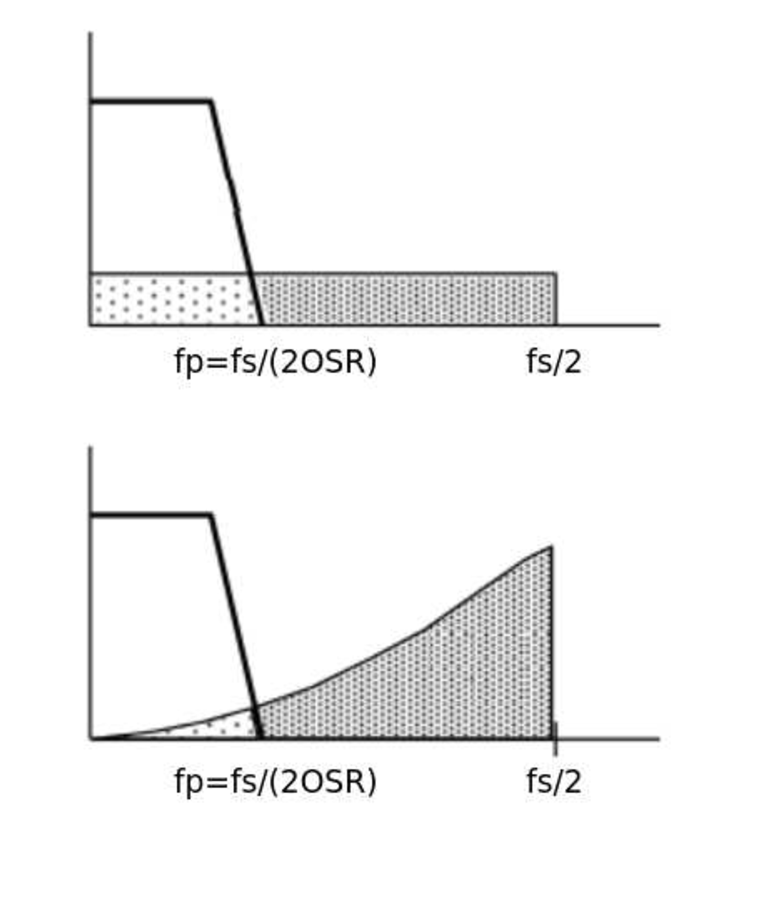
\includegraphics[width=1.7in]{Noise_Shaping.eps}
\caption{Arriba Oversampling. Abajo Oversampling+Noise Shapping}
\label{fig:NS}
\end{figure}

La topolog\'ia de un ADC sigma delta está representada en el diagrama en bloques de la Fig.~\ref{fig:SDTD}. La adición de ruido $N(z)$ es la modelización del ruido de cuantización. Analizando el diagrama, se puede obtener que:

\begin{align}
H_x(z)=\frac{H(z)}{1+H(z)} \qquad
H_n(z)=\frac{1}{1+H(z)}
\end{align}

donde $H_x$ y $H_n$ son las transferencias para la señal y para el ruido respectivamente. Siendo $H(z)$ un filtro pasabajos, $H_x(z)$ también será un filtro pasabajos (mientras sea $H(z)$ en la banda de paso mayor a 1) y $H_n(z)$ un filtro pasa altos. De esta forma se obtiene el \textit{Noise Shaping}.

\begin{figure}[!t]
\centering
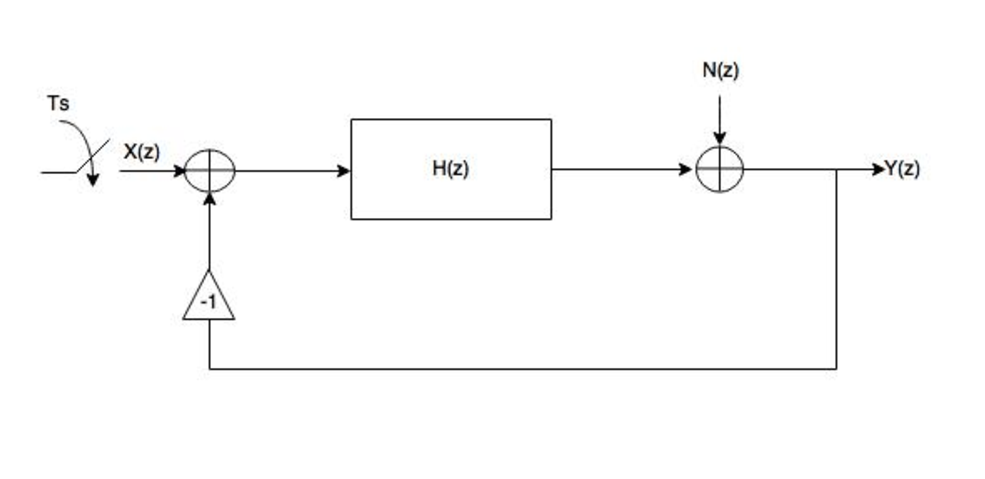
\includegraphics[height=1in]{Sigma-Delta_Tiempo_Discreto.eps}
\caption{Diagrana en bloques del modulador $\Sigma\Delta$}
\label{fig:SDTD}
\end{figure}

Para el desarrollo del proyecto, se utilizó el kit de desarrollo Mojo v3 el cual posee una \textit{FPGA Xilinx Spartan6}. En la Fig.~\ref{fig:DBADC} se resume el sistema completo, donde el filtro CIC es un filtro de decimación que utiliza pocos recursos de la FPGA. Este realiza una decimación de 512 veces, mientras que el filtro FIR decima 4, dando un factor de decimación total de 2048 veces.
%\hfill mds
%\hfill January 11, 2007

\begin{figure}[!t]
\centering
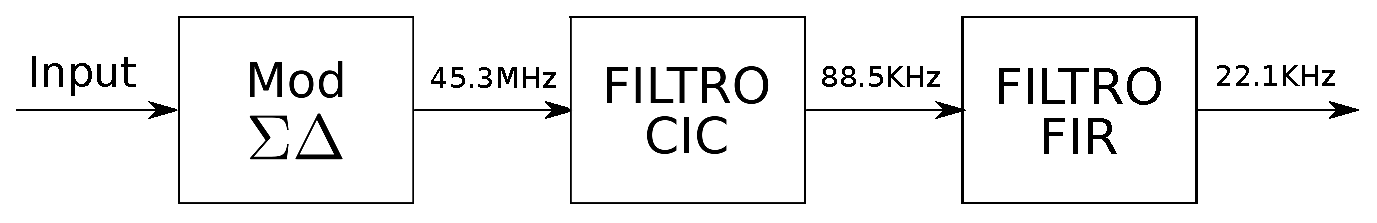
\includegraphics[width=3.5in]{Diagrama_Sistema_ADC.eps}
\caption{Diagrama en bloques del ADC}
\label{fig:DBADC}
\end{figure}

\subsection{Modulador $\Sigma\Delta$ en tiempo discreto}
Basado en el diagrama en bloques de la figura \ref{fig:SDTD}, un modulador de primer orden puede modelizarse con la siguiente transferencia:

\begin{align}
H(z)=\frac{z^{-1}}{1-z^{-1}}
\end{align}
De esto se obtiene que:
\begin{align}
H_x(z)=z^{-1} \qquad
H_n(z)=1-z^{-1}
\end{align}

Por lo tanto, la transferencia para la señal es simplemente un retardo, y la del ruido consta de la diferencia entre la muestra actual y la anterior.
Para implementar un filtro de orden k se suele recurrir a que su transferencia esté dada por:

\begin{align}
H_n(z)=\left( 1-z^{-1}\right)^{k}
\end{align}

\subsection{Ruido de cuantizaci\'on}
Suponiendo el ruido de cuantización como ruido blanco uniformemente distribuido entre -$\Delta$/2 y $\Delta$/2, siendo $\Delta$ el alto del escal\'on de cuantización se tiene que \cite{Tesis:Hellman}:

\begin{align}
S_q(f) &= \frac{\Delta^{2}}{12f_s}\\
P_{q}(f) &=\int\limits_{-f_s/2}^{f_s/2}S_q(f) \, |H_n(f) \times H_D(f)|^{2} df
\end{align}

Donde $S_q,P_q$ y $H_D$ son la densidad espectral de potencia de ruido, la potencia de ruido de cuantizaci\'on a la salida, y la transferencia del filtro digital respectivamente.
Teniendo en cuenta un filtro digital ideal con corte en $f_p$, y un modulador de orden k se obtiene que la relaci\'on se\~nal a ruido de cuantizaci\'on en funci\'on del \textit{oversampling ratio}
\footnote[1]
{
Se lo obtiene teniendo en cuenta que en el integrando para $OSR\gg 1$ es $f\leq f_p\ll f_s$ y $|H_n(e^{j2 \pi \frac{f}{f_s}})|^{2}= \sin(\pi \frac{f}{f_s})^{2k} \approx (\pi\frac{f}{f_s})^{2k}$ y que la potencia un seno de plena escala es $P_{sin}=\frac{1}{2} [(2^N-1)\frac{\Delta}{2}]^{2}$.
Usualmente aparece la formula con $2^{N}-1\approx2^N$.
} es:

\begin{align}
SQNR &\approx 1.76+20\,log_{10}(2N-1)+10\,(2k+1)\,log_{10}OSR\nonumber\\
&\quad
+10\,log_{10}(2k+1)-20k\,log_{10}\pi \\
OSR&=\frac{fp}{fs/2}
\end{align}

En la Fig.~\ref{fig:SQNR} se ilustra el resultado.

\begin{figure}[!t]
\centering
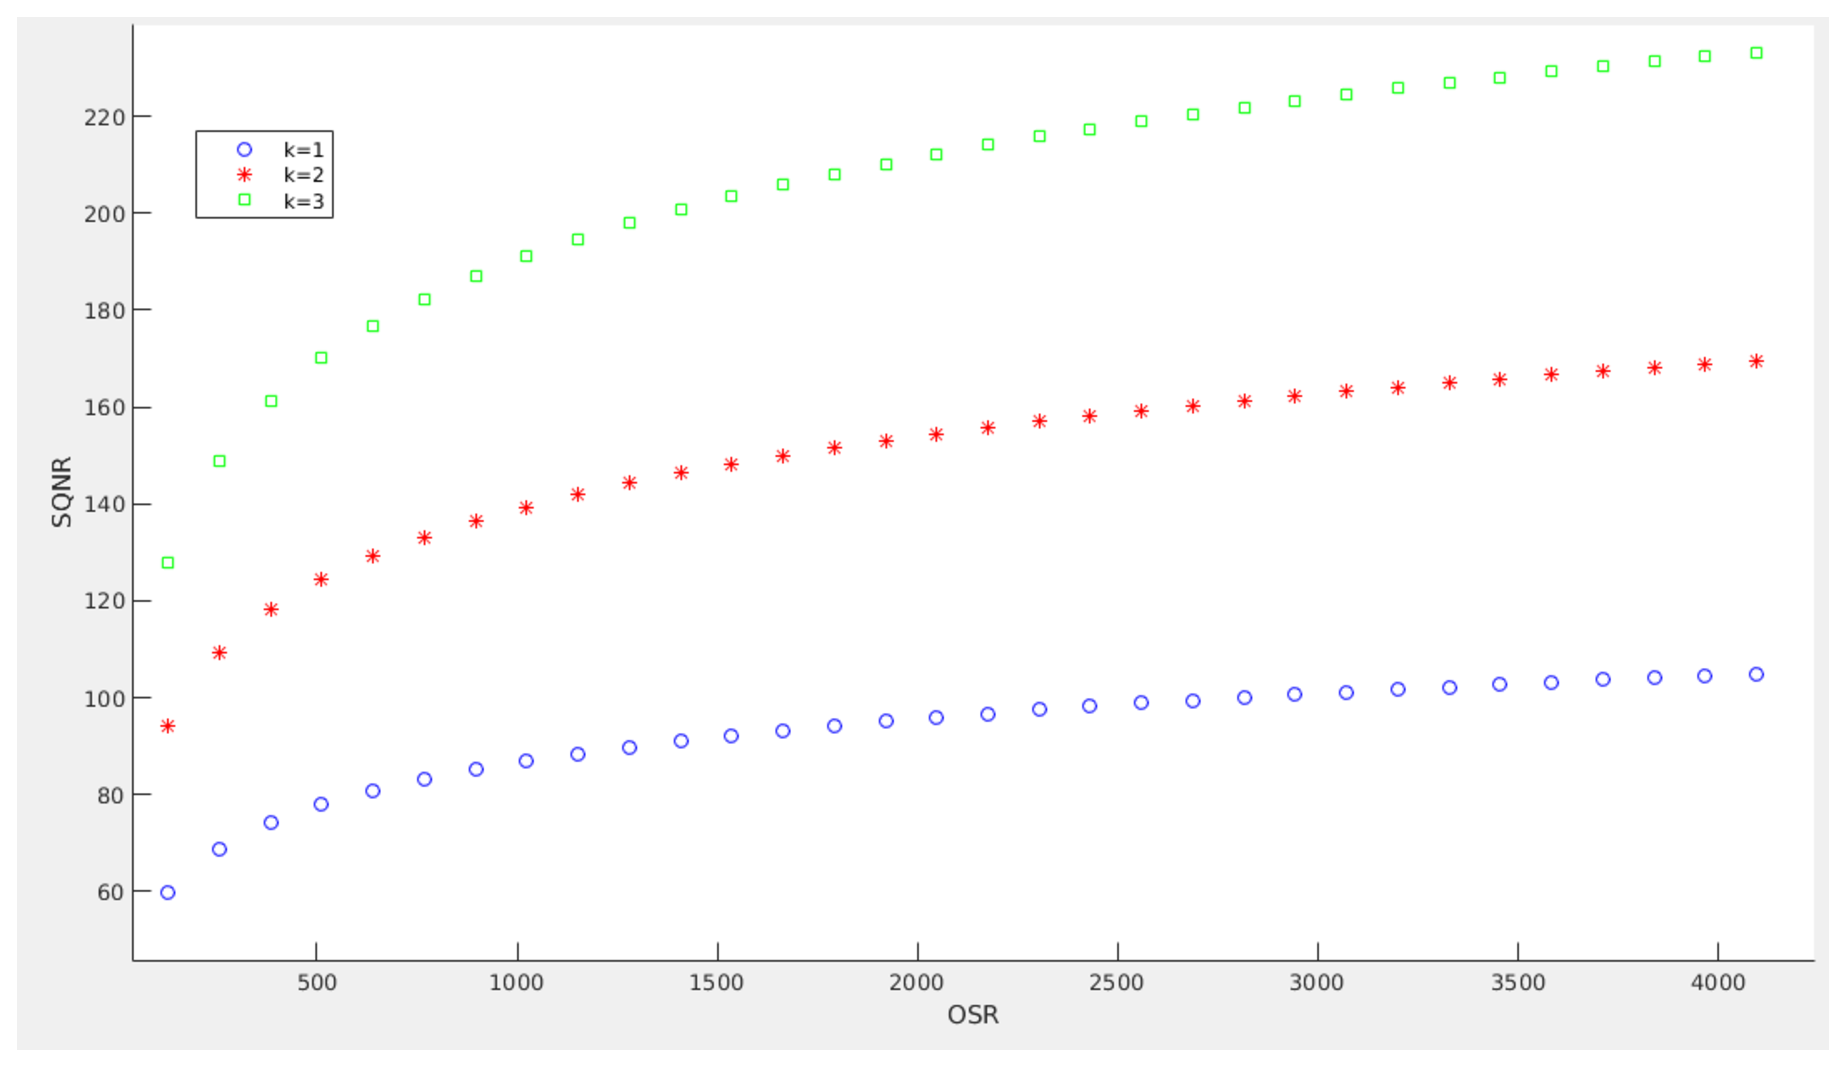
\includegraphics[width=3.5in]{SQNR_ideal_segun_OSR}
%\def\svgwidth{2.5in}
%\input{Noise_Shaping2.eps}
% where an .eps filename suffix will be assumed under latex, 
% and a .pdf suffix will be assumed for pdflatex; or what has been declared
% via \DeclareGraphicsExtensions.
\caption{SQNR en funci\'on de OSR para moduladores de diferente orden}
\label{fig:SQNR}
\end{figure}
%\subsubsection{Subsubsection Heading Here}
%Subsubsection text here.


% An example of a floating figure using the graphicx package.
% Note that \label must occur AFTER (or within) \caption.
% For figures, \caption should occur after the \includegraphics.
% Note that IEEEtran v1.7 and later has special internal code that
% is designed to preserve the operation of \label within \caption
% even when the captionsoff option is in effect. However, because
% of issues like this, it may be the safest practice to put all your
% \label just after \caption rather than within \caption{}.
%
% Reminder: the "draftcls" or "draftclsnofoot", not "draft", class
% option should be used if it is desired that the figures are to be
% displayed while in draft mode.
%
%\begin{figure}[!t]
%\centering
%\includegraphics[width=2.5in]{myfigure}
% where an .eps filename suffix will be assumed under latex, 
% and a .pdf suffix will be assumed for pdflatex; or what has been declared
% via \DeclareGraphicsExtensions.
%\caption{Simulation Results}
%\label{fig_sim}
%\end{figure}

% Note that IEEE typically puts floats only at the top, even when this
% results in a large percentage of a column being occupied by floats.


% An example of a double column floating figure using two subfigures.
% (The subfig.sty package must be loaded for this to work.)
% The subfigure \label commands are set within each subfloat command, the
% \label for the overall figure must come after \caption.
% \hfil must be used as a separator to get equal spacing.
% The subfigure.sty package works much the same way, except \subfigure is
% used instead of \subfloat.
%
%\begin{figure*}[!t]
%\centerline{\subfloat[Case I]\includegraphics[width=2.5in]{subfigcase1}%
%\label{fig_first_case}}
%\hfil
%\subfloat[Case II]{\includegraphics[width=2.5in]{subfigcase2}%
%\label{fig_second_case}}}
%\caption{Simulation results}
%\label{fig_sim}
%\end{figure*}
%
% Note that often IEEE papers with subfigures do not employ subfigure
% captions (using the optional argument to \subfloat), but instead will
% reference/describe all of them (a), (b), etc., within the main caption.


% An example of a floating table. Note that, for IEEE style tables, the 
% \caption command should come BEFORE the table. Table text will default to
% \footnotesize as IEEE normally uses this smaller font for tables.
% The \label must come after \caption as always.
%
%\begin{table}[!t]
%% increase table row spacing, adjust to taste
%\renewcommand{\arraystretch}{1.3}
% if using array.sty, it might be a good idea to tweak the value of
% \extrarowheight as needed to properly center the text within the cells
%\caption{An Example of a Table}
%\label{table_example}
%\centering
%% Some packages, such as MDW tools, offer better commands for making tables
%% than the plain LaTeX2e tabular which is used here.
%\begin{tabular}{|c||c|}
%\hline
%One & Two\\
%\hline
%Three & Four\\
%\hline
%\end{tabular}
%\end{table}


% Note that IEEE does not put floats in the very first column - or typically
% anywhere on the first page for that matter. Also, in-text middle ("here")
% positioning is not used. Most IEEE journals/conferences use top floats
% exclusively. Note that, LaTeX2e, unlike IEEE journals/conferences, places
% footnotes above bottom floats. This can be corrected via the \fnbelowfloat
% command of the stfloats package.

\section{Modulador $\Sigma\Delta$ en tiempo continuo}

A diferencia del modulador $\Sigma\Delta$ en tiempo discreto, el muestreo se realiza dentro del modulador, luego de la cuantización. Dicho cambio se aprecia en la Fig.~\ref{fig:SDTC} de la cual que se puede obtener la siguiente transferencia para la señal y para el ruido:

%En la Fig.~\ref{fig:SDTC} donde se reemplazó el cuantizador por su modelo de ruido aditivo, las transferencias para la se\~nal y para el ruido quedan:

\begin{align}
H_x(e^{sT_s}) &= \frac{H(s)}{1+H_{eq}(e^{sT_s})} \\
H_n(z) &= \frac{1}{1+H_{eq}(z)} \\
h_{eq}[n] &= (h\ast h_{DAC})(nT_s)
\end{align}

Donde la respuesta de lazo equivalente en tiempo discreto $H_{eq}(z)$ se la obtiene por la transformaci\'on de invarianza al impulso\cite{DSP:Pro-Man} de $H(s)H_{DAC}(s)$ dada por (11). Para un retenedor de orden cero queda como:

\begin{align}
 H_{DAC}(s)&=\frac{1-e^{-sT_s}}{s}\\
 Z^{-1}(\frac{H_{eq}(z)}{1-z^{-1}})[n]&=L^{-1}(\frac{H(s)}{s})(nT_s)
\end{align}

Partiendo del modulador de primer orden en tiempo discreto y con la anterior transformaci\'on se obtiene:

\begin{align}
 H(s)&=\frac{1}{sT_s}\\
 H_x(e^{sT_s})&= \frac{1-e^{-sT_s}}{s}
\end{align}

Considerando que el filtro $H(s)$ es un integrador, la trasferencia para la se\~nal es un pasabajos con ceros en múltiplos de $f_s$, lo cual reduce notablemente el alias en la banda de paso.

\begin{figure}[!t]
\centering
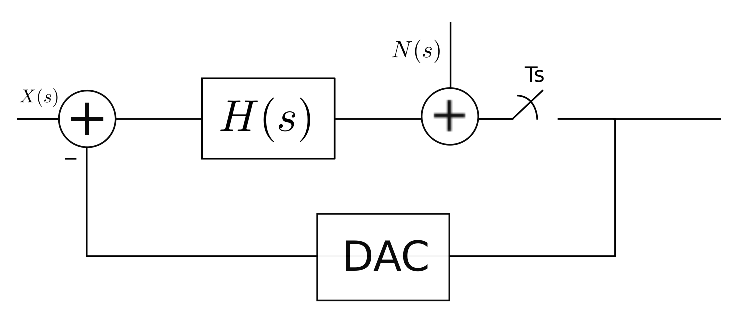
\includegraphics[height=1in]{Sigma-Delta_Tiempo_Continuo}
\caption{Diag. en bloques del modulador $\Sigma\Delta$ en tiempo continuo}
\label{fig:SDTC}
\end{figure}

\subsection{Implementaci\'on}

\begin{figure}[!t]
\centering
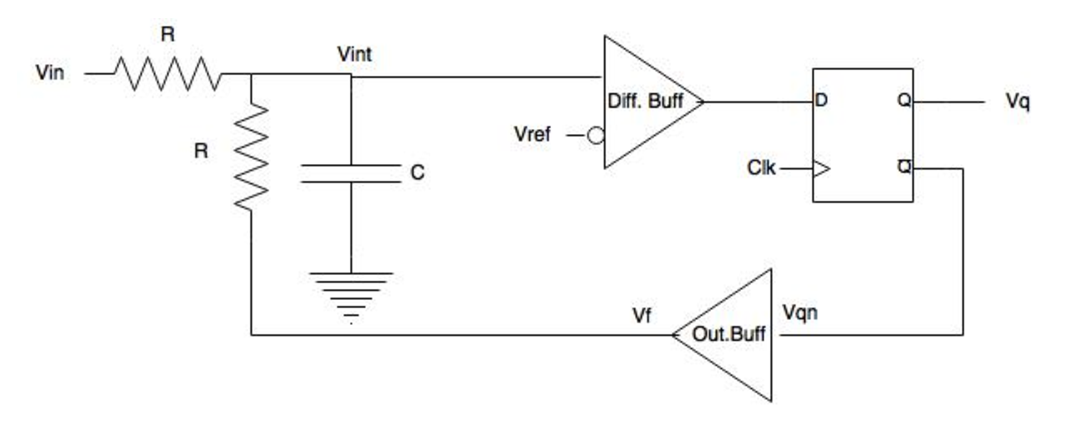
\includegraphics[width=3in]{Sigma-Delta_RC}
\caption{Circuito utilizado para el modulador $\Sigma\Delta$}
\label{fig_SDRC}
\end{figure}

La topolog\'ia m\'as sencilla para la implementaci\'on es el modulador RC (Fig.\ref{fig_SDRC}). La cuantificaci\'on es realizada por una entrada LVDS de la FPGA\cite{Sp6-IO} utilizada com\'unmente para comunicaciones diferenciales y posteriormente la discretizaci\'on temporal es realizada por un flip-flop. La tensi\'on de entrada posee un rango de 0v a la alimentación de la fpga (3.3v), y la referencia está a mitad de escala (1.65v).  Haciendo un breve an\'alisis del circuito, se ve que la tensi\'on en la entrada del comparador tomar\'a valores cercanos a la referencia, y como respecto a \'esta la amplitud de la salida ser\'a 1.65v, el comparador presenta una ganancia para la se\~nal. Esto es lo que hace posible funcionar al modulador pasivo, ya que el filtro debe tener ganancia mayor a uno. Generalmente a esta ganancia se la estima pasivando la entrada de señal, lo cual provoca una oscilación de la mitad de la frecuencia de \textit{clk}. La ganancia del comparador ser\'ia :
\begin{align}
G(s)=\frac{1}{|H(j\pi f_s)|}
\end{align}
Realmente, esta ganancia está correlacionada con Vin provocando alinealidades en el sistema.\\
La transferencia del filtro RC es:
\begin{align}
H(s)=\frac{1}{2+sCR}
\end{align}
La transferencia a lazo abierto por lo tanto es $G*H(s)$. 
Se obtiene la transferencia de lazo equivalente como:
\begin{align}
H_{eq}(z)=\frac{1}{2}\frac{1-e^{-\frac{2}{RC}T_s}}{1-e^{-\frac{2}{RC}T_s}z^{-1}}
\end{align}
El PLL de la fpga fue ajustado a 45.3125MHz, y al sistema digital se lo hizo decimar 2048 veces, por lo que a la salida se tendrán 22.13 Ksps. El valor de resistencia usada fue de 150k, y el capacitor de 470pF (corte en 4.3kHz).
Con esto se puede graficar las transferencias para la señal y para el ruido con las fórmulas antes indicadas (Fig.~\ref{fig:Resp_mod}). Observando la transferencia para la señal, se ve que el ripple es despreciable. Luego con la transferencia para el ruido en la banda de paso, se estimó el ENOB realizando una integraci\'on num\'erica que dio como resultado 13,6. Por último, se observa que la primer zona de alias tiene un m\'aximo de -72dB.

\begin{figure}[!t]
\centering
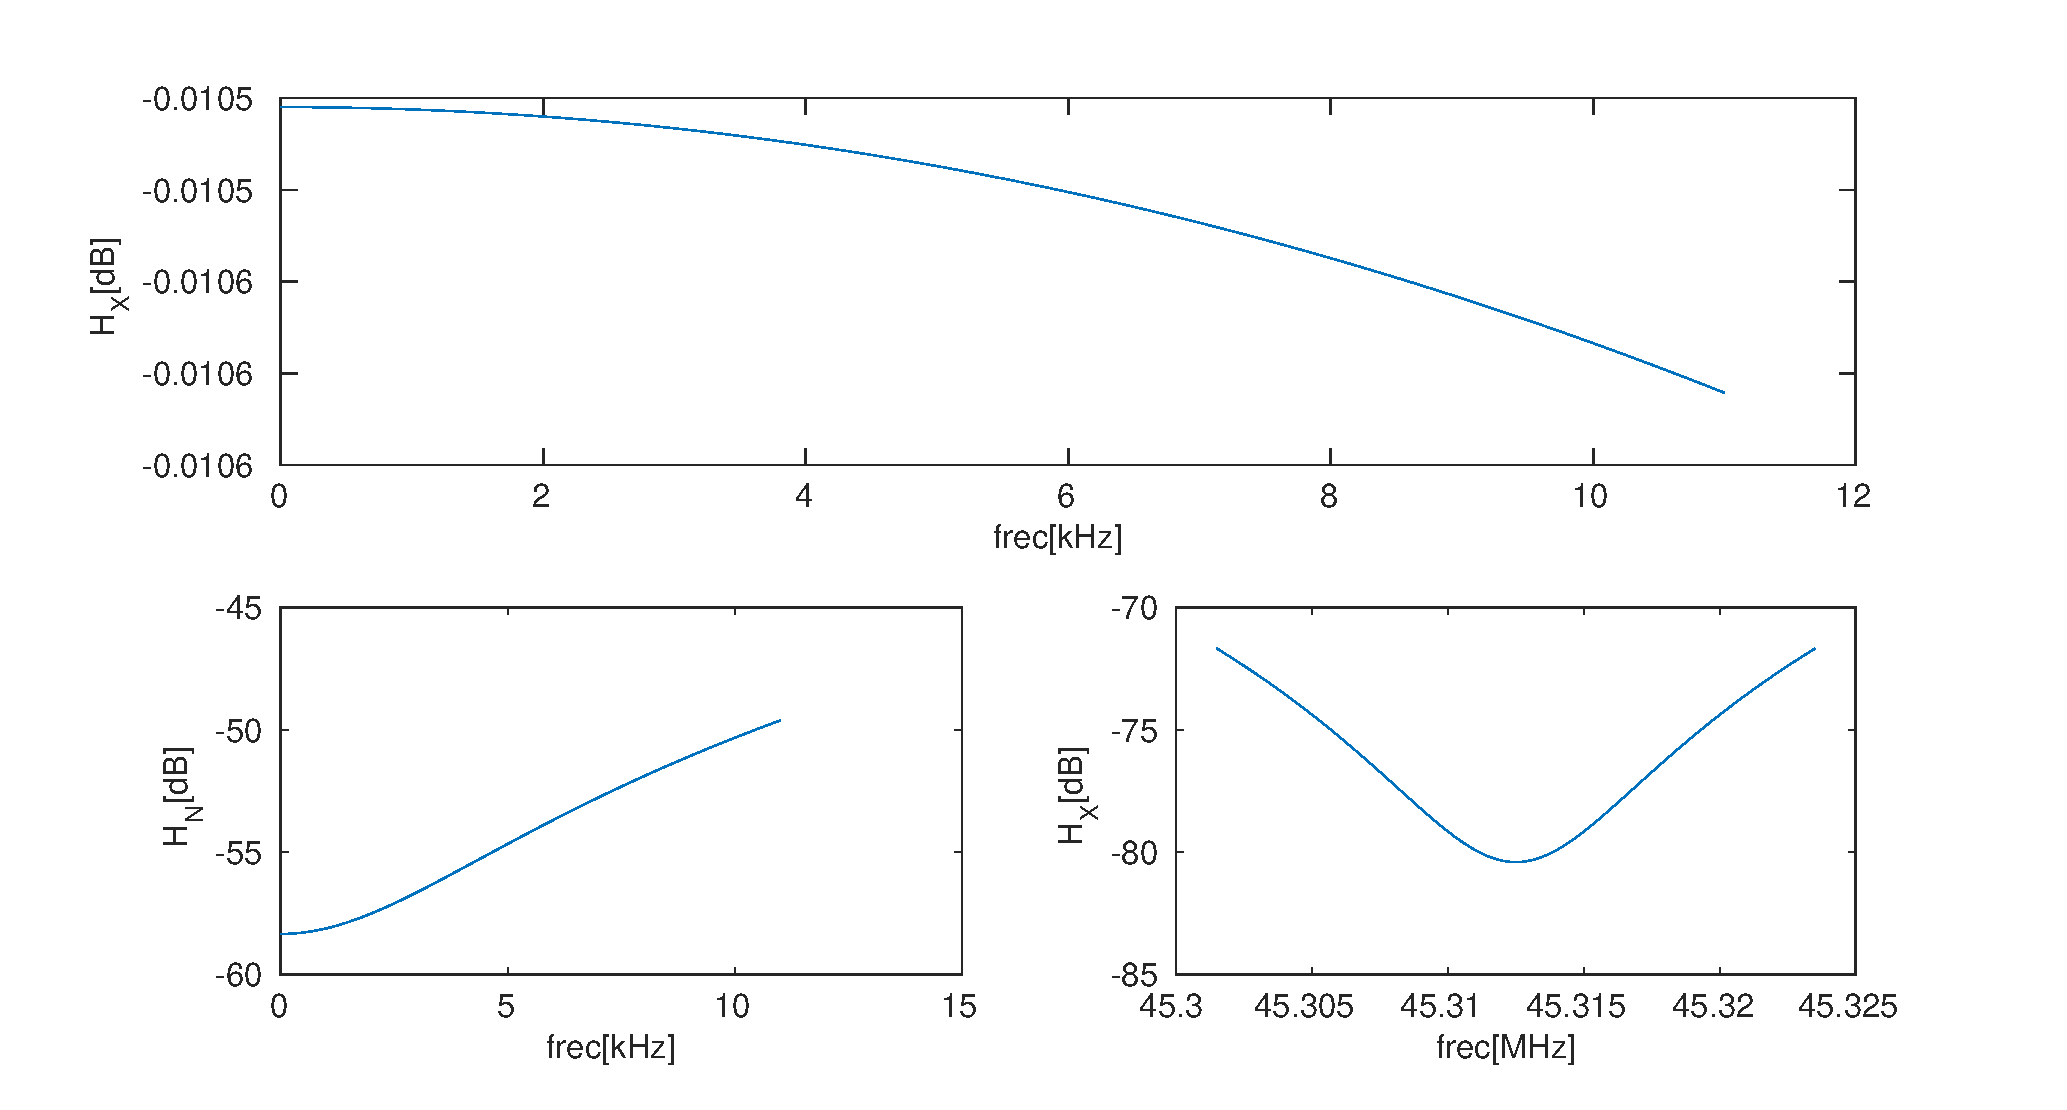
\includegraphics[width=3.5in]{Respuesta_Modulador_Combinada}
\caption{Arriba: Transferencia para la se\~nal en la banda de paso. Abajo: Transferencia para el ruido (izquierda) y primer zona de alias para la se\~nal}
\label{fig:Resp_mod}
\end{figure}

\subsection{Simulaci\'on}


Para realizar la simulación del modulador, se modelizó el comparador incluyendo efectos de histéresis y adición de ruido sobre la tensión de referencia. En la simulaci\'on no se incluyeron las caracter\'isticas el\'ectricas de los buffers de entrada y salida de la \textit{FPGA}. En la Fig.~\ref{fig:Sim_mod} se ve una simulaci\'on de la respuesta para una señal de 1kHz. En esta se ve que la salida del integrador RC tiene una oscilación pico a pico 2mV, lo que significa una ganancia de señal G=1650. Al resimular el ENOB del modulador RC con esta ganancia se obtiene un resultado de 10.93 (el alias se mantiene en -72dB).

\begin{figure}[!t]
\centering
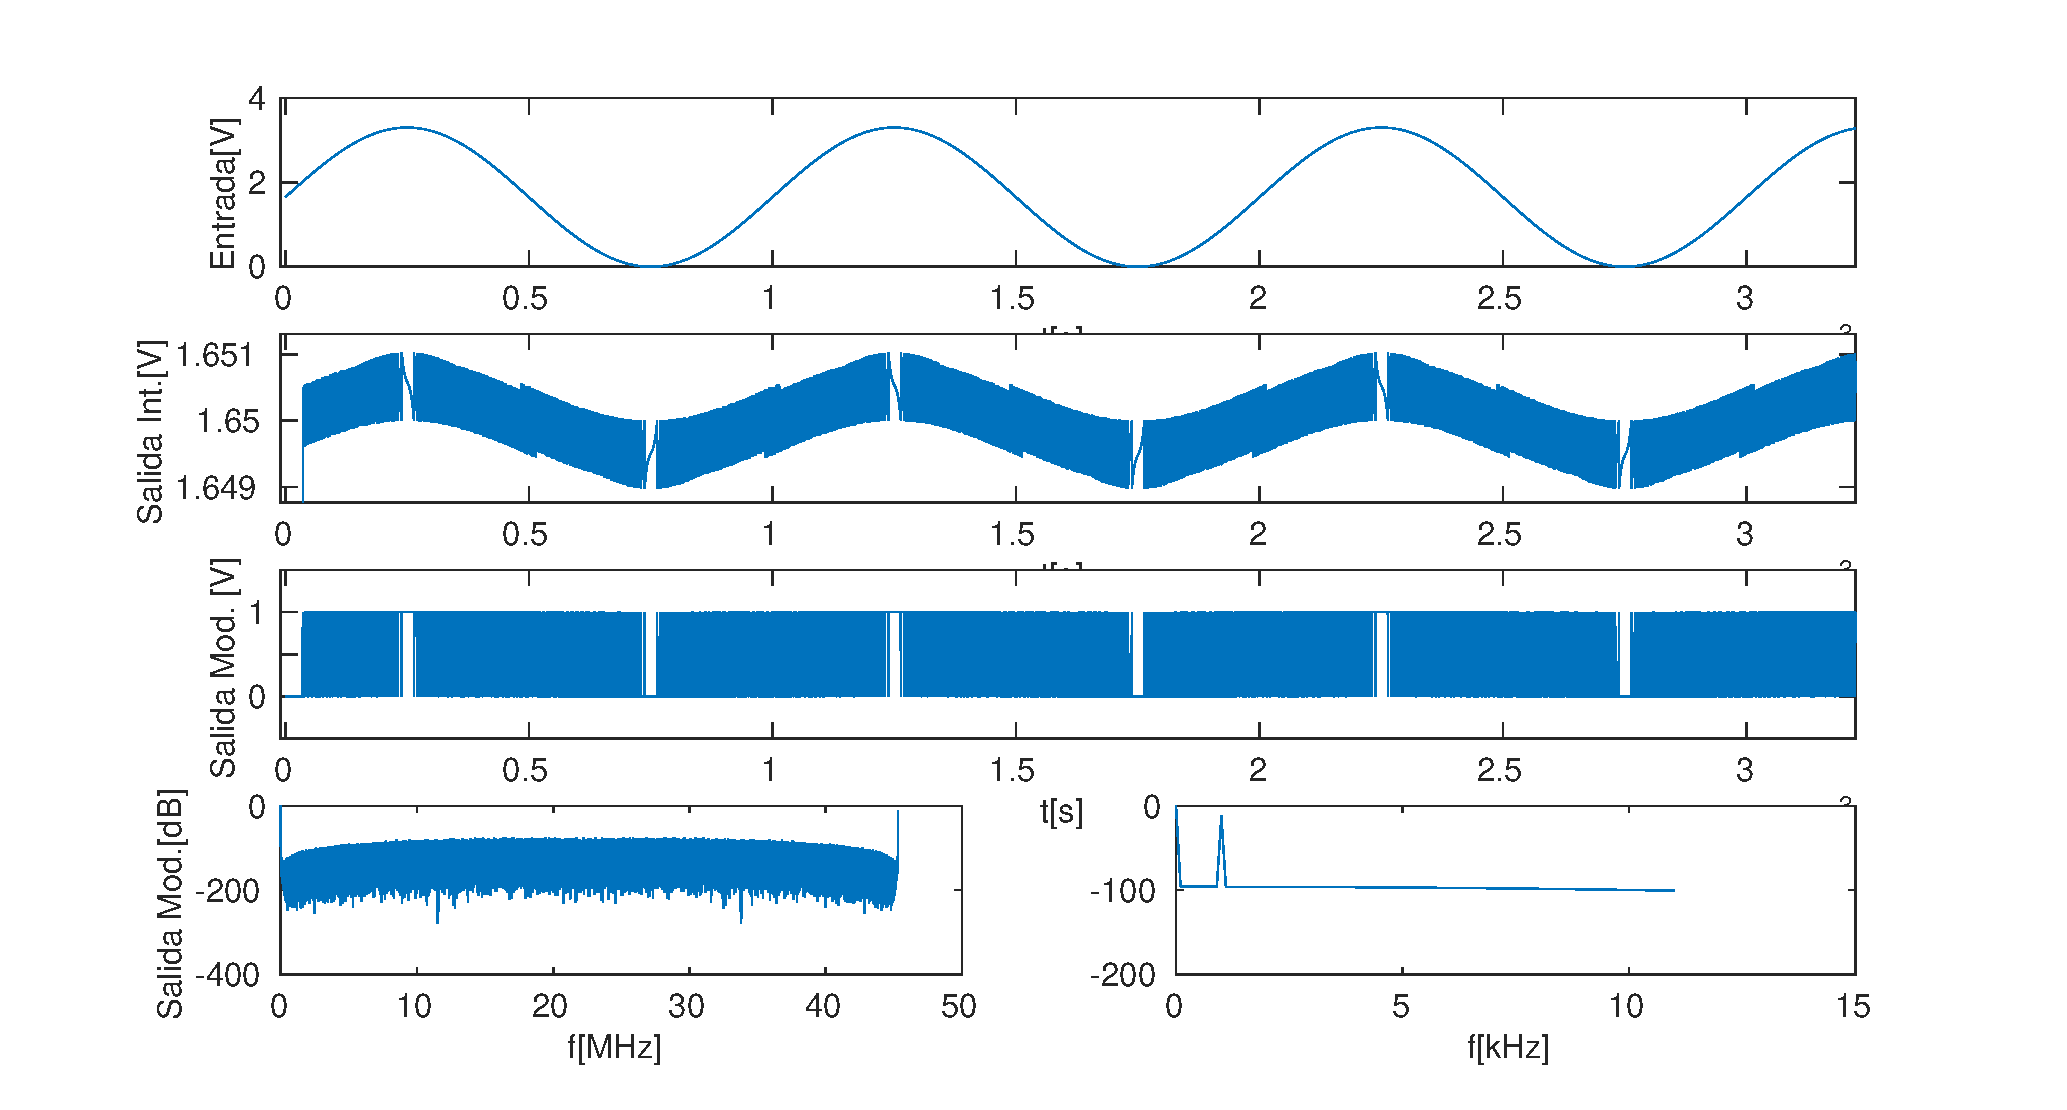
\includegraphics[width=3.5in]{Simulacion_Modulador}
\caption{De arriba hacia abajo: Señal de entrada, señal en la entrada del comparador, señal de salida del modulador,  espectro de la salida donde se visualiza el \textit{Noise Shaping} (izquierda), zoom en la banda de paso (derecha).}
\label{fig:Sim_mod}
\end{figure}



\section{Filtro decimador CIC}

\begin{figure}[!b]
	\centering
	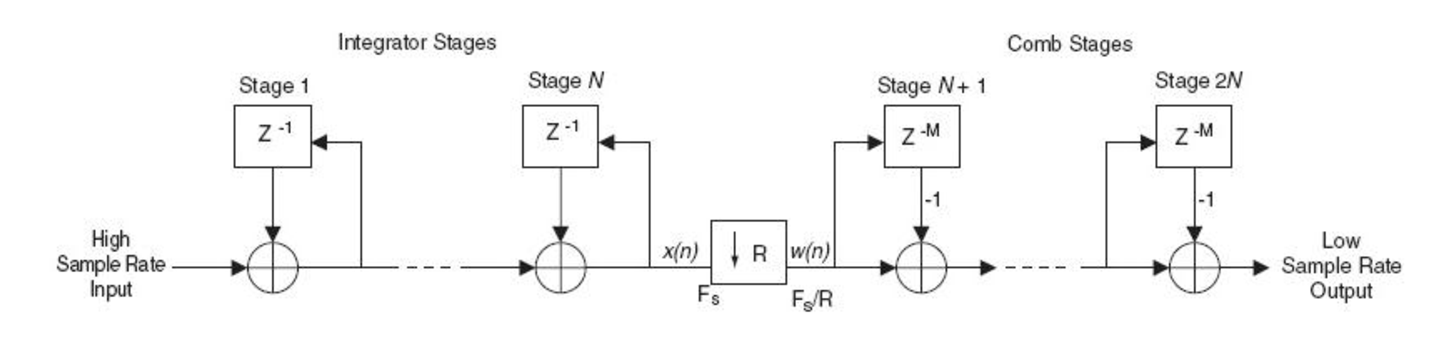
\includegraphics[width=3.5in]{CIC_Topologia}
	\caption{Estructura de un filtro CIC}
	\label{fig:CIC_top}
\end{figure}

El filtro CIC (Cascaded Integrator-Comb) presentado por Hogenauer en 1981\cite{CIC:Hog},  es un filtro pasa bajos que tiene como principal caracter\'istica su eficiente implementaci\'on (ver Fig.~\ref{fig:CIC_top}), logrando bajar la frecuencia de trabajo con un filtro sencillo que presenta poco alias en el ancho de banda de interés.

Se puede observar que cada par de acumulador (a la izquierda del decimador), y \textit{comb} (a la derecha), forman un filtro de media m\'ovil con ventana de ancho R*M. La transferencia de \'este es:

\begin{align}
H_{CIC}(z)= \left( H_I(z) H_c(z)\right)& ^{N}=\left( \frac{1-z^{-RM}}{1-z^{-1}}\right) ^N\\
\left| H_{CIC}(e^{j2\pi\frac{f}{R}})\right| &=\left| \frac{\sin(\pi M\,f)}{\sin(\pi \frac{f}{R})}\right| ^{N}
\end{align}

siendo f la frecuencia normalizada al downsampling rate.\\


Se observa que los ceros del CIC se producen en los m\'ultiplos de la low sampling rate, es decir, las zonas de alias. El m\'aximo alias es en f=1-fp (normalizado), y se puede tener s\'olo en cuenta este valor ya que el aporte de los siguientes l\'obulos es mucho menor, considerando fp como el ancho de banda del filtro ideal que va a continuación del filtro CIC.

\subsection{Implementaci\'on y simulaci\'on}
El filtro CIC se determin\'o de 6 etapas, para el cual se utilizaron 12 sumadores de 55 bits. Para reducir el tiempo combinacional y poder tener una frecuencia de trabajo mayor, cada etapa fue registrada. A su vez, se implement\'o entre las etapas el bloque de decimaci\'on con un factor de 512. El retraso en los \textit{comb} se determin\'o M=1. Las salidas del CIC son almacenadas en una Dual-Port BlockRam\cite{Sp6-BR} la cual tiene la caracter\'istica de poder realizar la lectura de dos datos de manera simultánea. Los datos almacenados en la misma fueron truncados a 16 bits para optimizar la síntesis. En la Fig.~\ref{fig:CIC_resp} se muestra la respuesta en la banda de paso, y la primer zona de alias. Se puede observar que hay una atenuación de 1.5dB en la banda de paso, y el alias que se producirá es de -100dB.

\begin{figure}[!t]
\centering
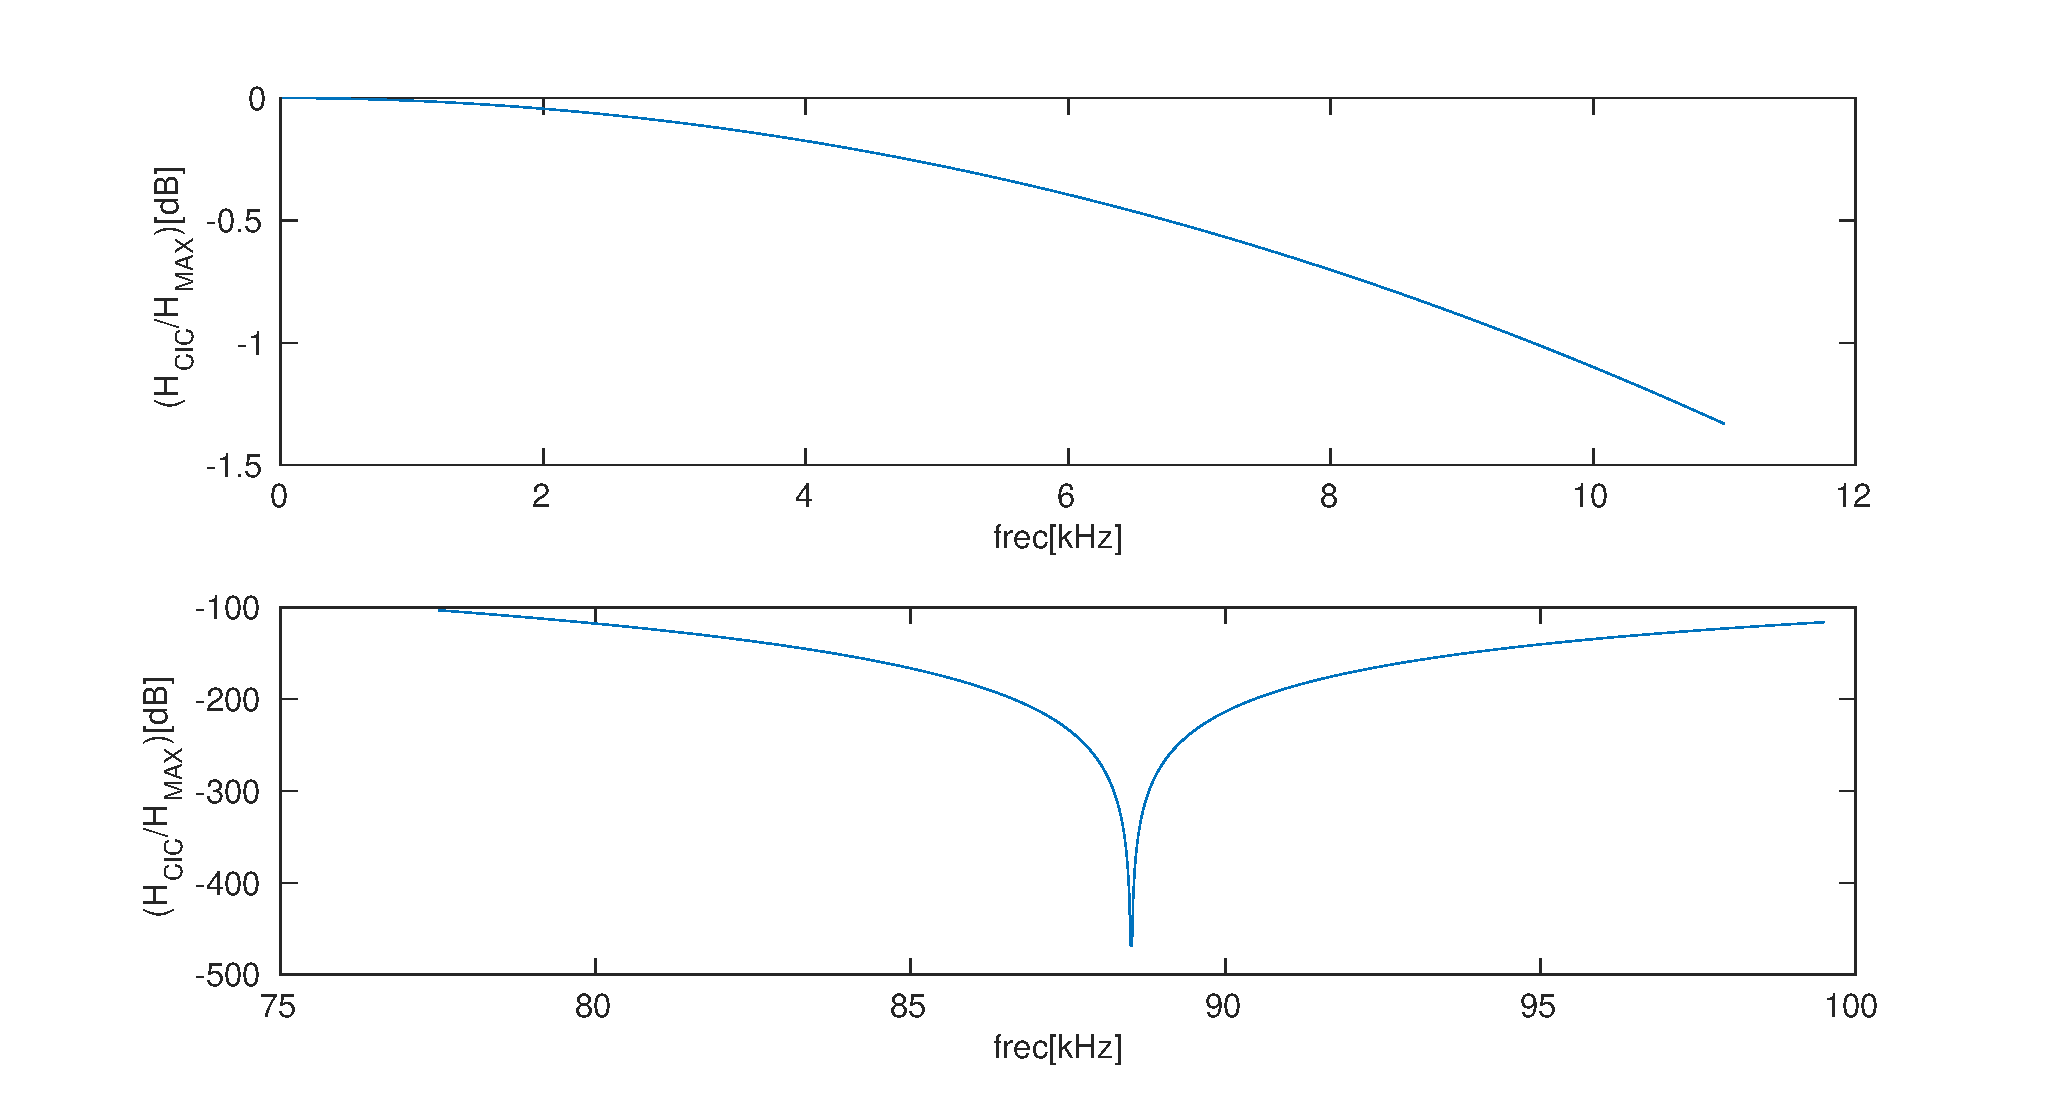
\includegraphics[width=3.5in]{Respuesta_CIC}
\caption{Respuesta del CIC: Banda de paso (Arriba) y primer zona de alias (Abajo)}
\label{fig:CIC_resp}
\end{figure}

\section{Filtro FIR}

El filtro FIR busca ecualizar la transferencia en la banda de paso del CIC (la cual no es plana), y eliminar el ruido de cuantizaci\'on fuera de la banda de interés antes de la 
decimaci\'on final. Se lo dise\~n\'o por el m\'etodo de sampleo y ventaneo con una ventana Kaiser, donde en la banda de paso se muestrea la inversa de la respuesta en frecuencia del filtro CIC usado y fuera de esta se determina con ceros\cite{FIR_Comp}. En la Fig.~\ref{fig:FIR_res} se muestra la respuesta del filtro FIR diseñado, que posee una atenuaci\'on de 80dB.
Para la implementación del FIR, se utiliz\'o la estructura de PreAdder-Multiplicador-Acumulador (Fig.~\ref{fig:FIR_top}) que posee los bloques \textit{DSP} de la \textit{FPGA}\cite{Sp6-DSP}. Se utiliz\'o un filtro FIR sim\'etrico de 256 coeficientes  con frecuencia de corte normalizada de 0.22. Al ser sim\'etrico, s\'olo es necesario almacenar la mitad de los coeficientes y tambi\'en se reduce a la mitad el c\'alculo al poder utilizar el preadder.  Posteriormente, se realiza una \'ultima decimaci\'on por un factor de 4, dando como resultante una decimaci\'on total de 2048. El resultado final fue truncado a 16 bits.


\newpage

\begin{figure}[!t]
	\centering
	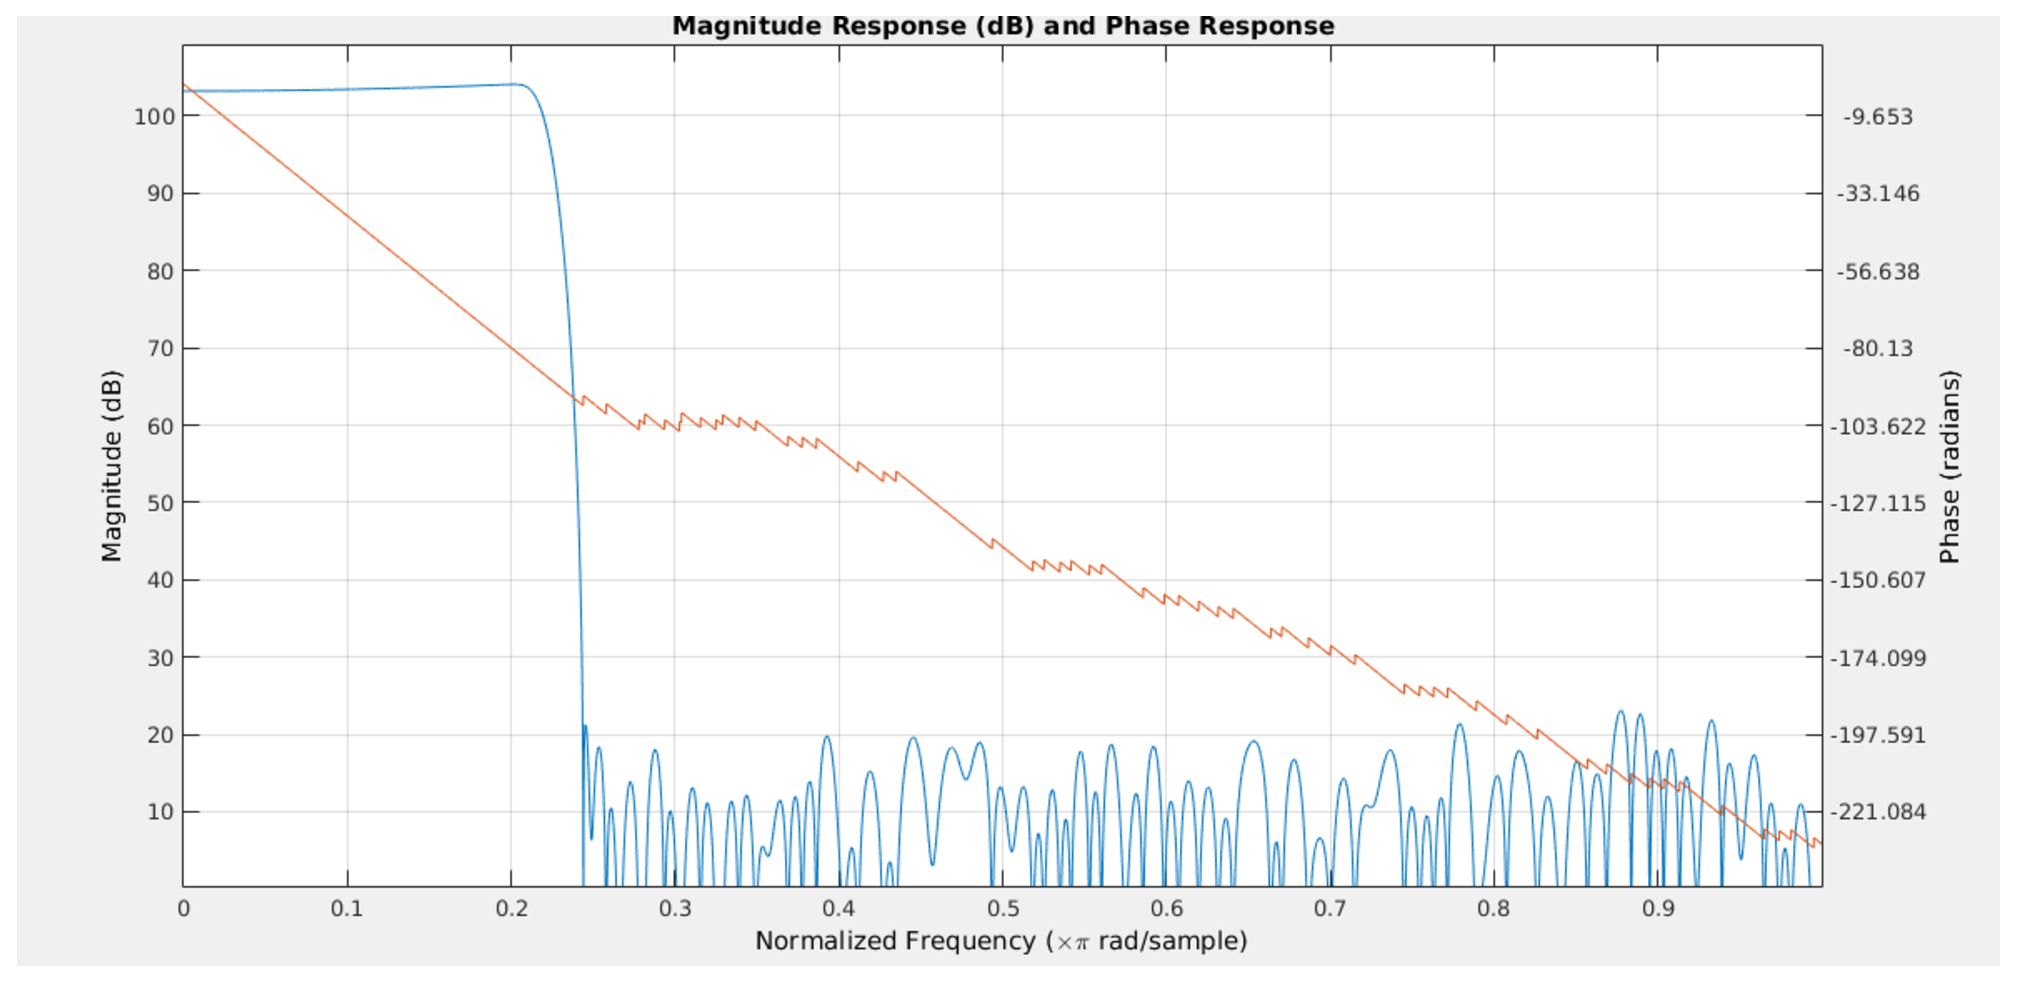
\includegraphics[width=3.5in]{Respuesta_FIR}
	\caption{Respuesta del FIR}
	\label{fig:FIR_res}
\centering
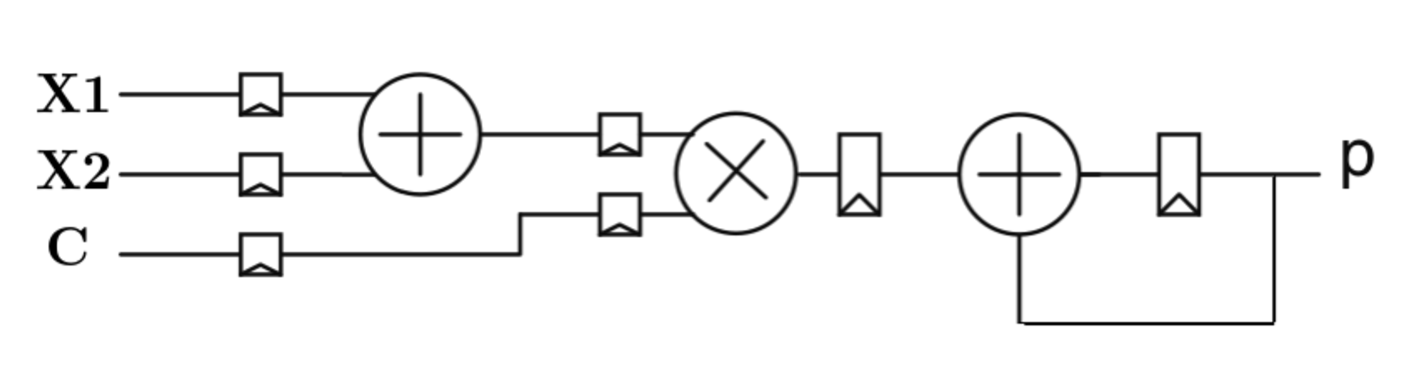
\includegraphics[width=3.5in]{FIR_Topologia}
\caption{Topolog\'ia usada en la implementaci\'on del FIR}
\label{fig:FIR_top}
\end{figure}


\begin{table}[!b]
	%% increase table row spacing, adjust to taste
	\renewcommand{\arraystretch}{1.3}
	% if using array.sty, it might be a good idea to tweak the value of
	% \extrarowheight as needed to properly center the text within the cells
	\caption{Resultado Simulaci\'on ENOB}
	\label{Tabla:sim}
	\centering
	%% Some packages, such as MDW tools, offer better commands for making tables
	%% than the plain LaTeX2e tabular which is used here.
	\begin{tabular}{|c|c|c|}
		\hline
		Frec. entrada & Frec. Fiteo & ENOB\\
		\hline
		1k & 999.99 & 11.17\\
		\hline
		2k & 2000.00 & 11.01\\
		\hline
		4k & 4000.00 & 10.68\\
		\hline
		8k & 8000.00 & 9.84\\
		\hline
		9k & 8999.99 & 9.56\\
		\hline
		10k & 9999.98 & 7.85\\
		\hline
	\end{tabular}
\end{table}

\section{Simulaci\'on}
Se simul\'o el modulador descripto previamente, as\'i como el filtro CIC y el FIR en Matlab\textregistered.
Durante las simulaciones, se realizaron pruebas de linealidad barriendo la entrada con una rampa de muy baja frecuencia y se pudo ver que el sistema posee un comportamiento totalmente lineal.
Tambi\'en se realizaron simulaciones barriendo en frecuencia para obtener la cantidad efectiva de bits. Sabiendo que los mismos estan definidos por: 
\begin{align}
ENOB = \dfrac{SINAD-1.73}{6.02}
\end{align}
se procedió a buscar un estimador para el SINAD (Razón entre la potencia de la Se\~nal y el ruido en conjunto con la distorsi\'on). Para ello, se excitó el sistema con una señal senoidal y se almacenaron los datos de la salida de la simulación. Posteriormente, se les realizó un \textit{fitting} con una función senoidal con tres grados de libertad (Amplitud, frecuencia y fase). Con esto, se obtuvo la función que mejor la aproxima la señal obtneida y se realizó una resta punto a punto para así, poder determinar la potencia del ruido y con ello, el SINAD. Con esto, se obtuvieron los bits efectivos resumidos en la Tabla~\ref{Tabla:sim}.


\section{Mediciones}

\begin{figure}[!b]
\centering
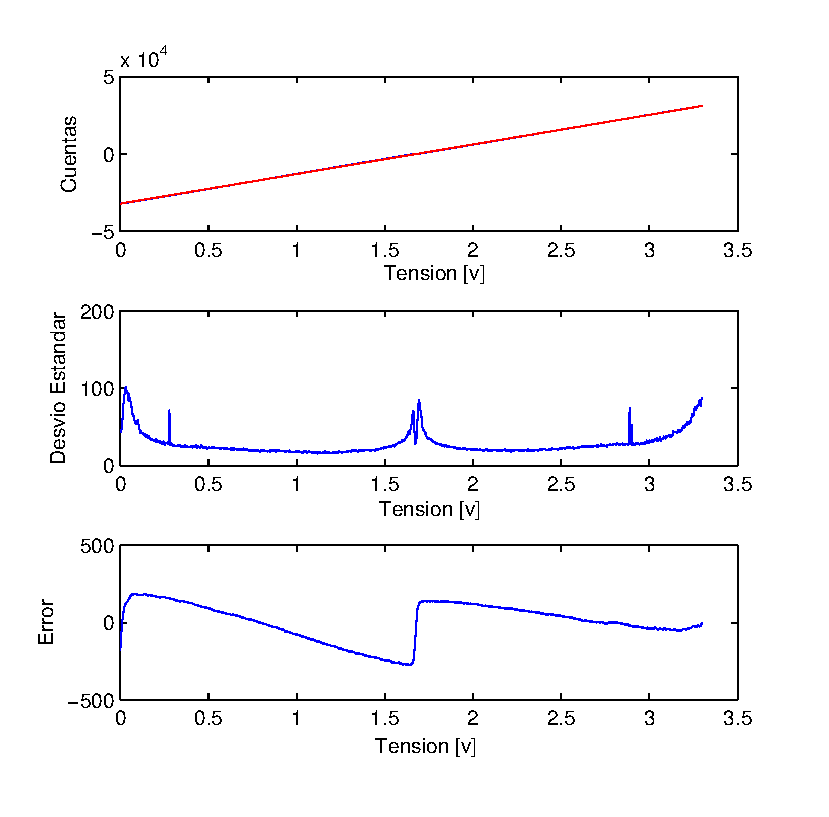
\includegraphics[width=3.5in]{Linealidad}
\caption{Arriba: Curva de linealidad (azul) y regresión lineal (roja). Medio: Desvío Estándar de las mediciones. Abajo: Error entre la curva de linealidad y regresión lineal}

\label{fig:lin}
	\centering
	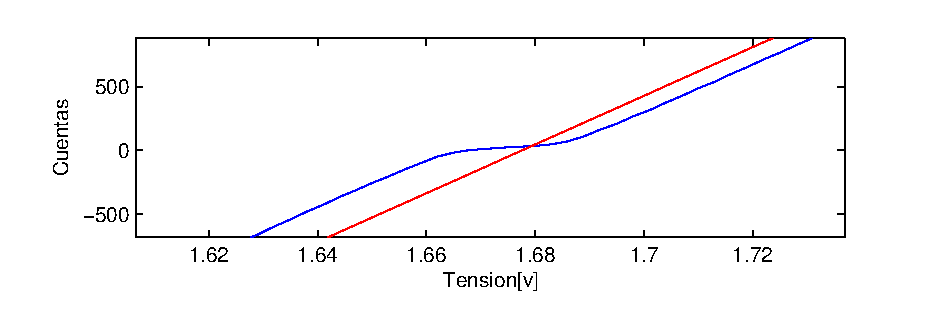
\includegraphics[width=3.5in]{Linealidad_codo}
	\caption{Ampliación del codo en la curva de linealidad. Curva de linealidad (azul), regresión lineal (rojo)}
	
	\label{fig:lincodo}
\end{figure}

Para realizar las mediciones se implementó una comunicaci\'on UART entre la \textit{FPGA} y la PC a 921600 baudios. El set de medici\'on const\'o de un generador de funciones Agilent 3352A\cite{AgilentWG}, controlado v\'ia TCP desde la computadora. La adquisición de datos, su almacenamiento y posterior análisis se realizó mediante la herramienta de cálculo Matlab\textregistered. \\Se llevaron a cabo tres mediciones: Linealidad, THD y ENOB.\\
Para realizar la medición de linealidad, se procedió a barrer todo el rango de tensión (0 a 3.3v) con un paso de 3mV obteniendo 1000 muestras por cada uno. Posteriormente, se realizó una regresión lineal de las muestras obteniendo las curvas representadas en la figura \ref{fig:lin}. Como se aprecia en la figura \ref{fig:lincodo}, la curva presenta una alinealidad significativa. Para análisis posteriores, se procedió a generar una curva de corrección para contrarrestar este efecto. Con tal fin, se generó una interpolación de la señal de error para poder tener $2^{16}$ valores para corregir.\\
Para el cálculo de THD y ENOB, se procedió a excitar el sistema con señales senoidales \textit{full-range} y se hizo un barrido en frecuencia entre 0 y 11KHz con pasos logarítmicos para los cuales se adquirieron un mínimo de 1000 muestras y con la restricción de tener un número entero de períodos de la señal senoidal, así evitar futuros problemas.
Una vez adquiridas las muestras, mediante el uso del periodograma con ventana de Kaiser, se realizaron las mediciones del THD. Para ello, conociendo la frecuencia de la fundamental (con la cual se excitó el sistema), se identificaron las armónicas y se determinó su potencia. Las cuales se reemplazaron en la siguiente expresión:
\begin{align}
THD = \dfrac{\sum_{i=1}^{M}P_i }{P_0}\cdot100
\end{align}
Siendo $P_0$ la potencia de la fundamental y $P_i$ la potencia de los respectivos armónicos.\\
Para la medición del ENOB, se realizó el mismo procedimiento llevado acabo en la simulación pero en este caso con datos adquiridos.\\
Estas mismas mediciones (ENOB y THD) se realizaron una segunda vez pero para los datos aplicando previamente la corrección obtenida durante el \textit{test} de linealidad. Como resultado, se obtuvieron las curvas trazadas en las figuras \ref{fig:ENOB} y \ref{fig:THD}, en azul representando las curvas con corrección y en rojo sin ella.
\begin{figure}[!t]
\centering
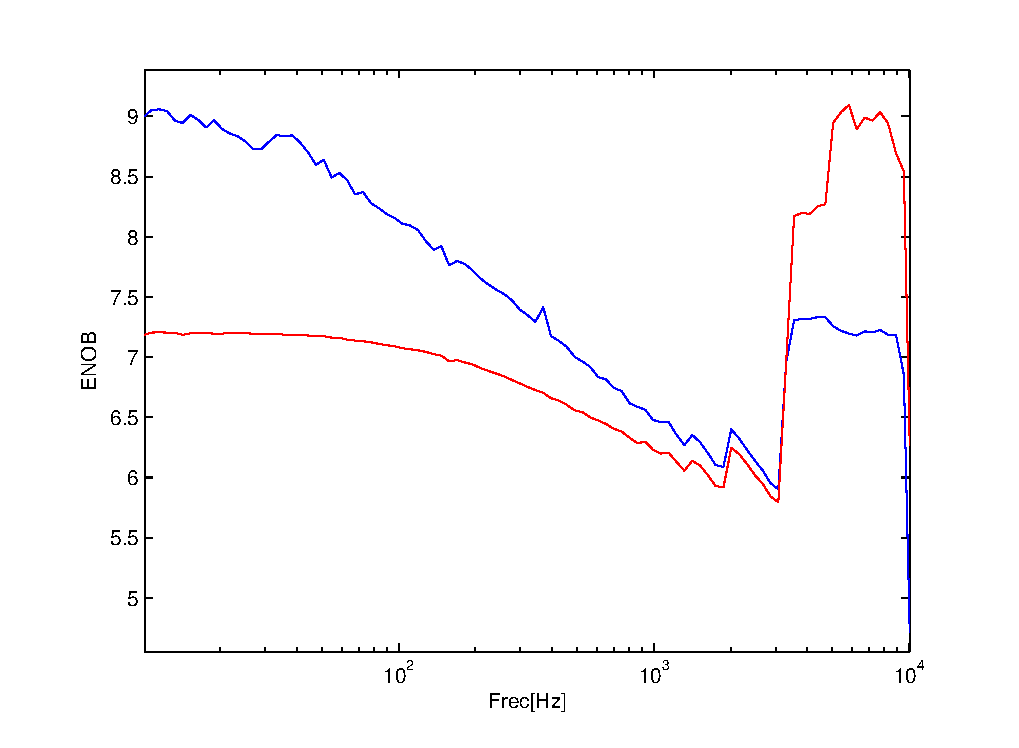
\includegraphics[height=2in]{Medicion_ENOB}
\caption{ENOB en funcion de la frecuencia. Azul: Corregida. Rojo: Sin Corregir}
\label{fig:ENOB}
\centering
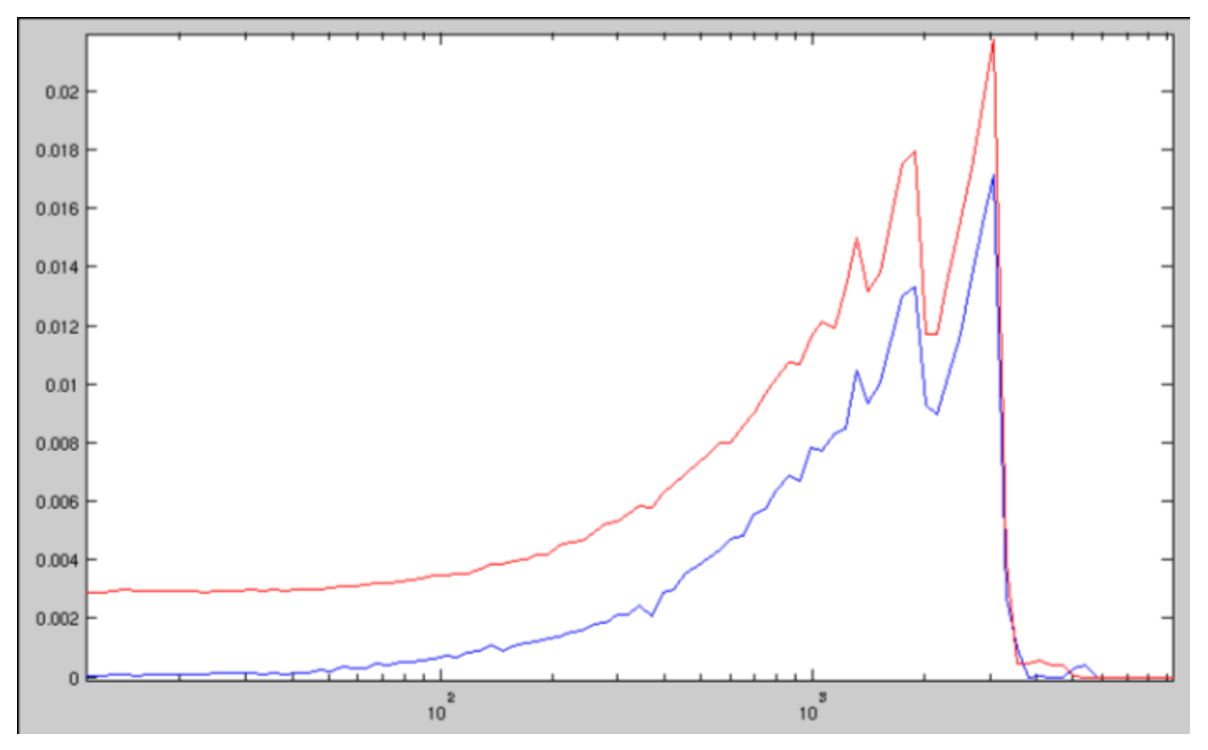
\includegraphics[height=2in]{Medicion_THD}
\caption{THD en función de la frecuencia. Azul: Corregida. Rojo: Sin Corregir}
\label{fig:THD}
\end{figure}



\section{Discusión y Conclusi\'ones}
Analizando las curvas obtenidas, podemos notar que el limitante de nuestro proyecto es la distorsión armónica generada en el modulador. Esta distorsión no fue percibida durante las simulaciones debido a que en la misma no se tuvieron en cuenta las características eléctricas de los componentes y de la \textit{FPGA}. Si se aplica la corrección digital al sistema, los resultados son prometedores en las bajas frecuencias alcanzando los 9 bits efectivos. Para frecuencias mayores a 100 Hz, esta corrección empieza a perder efectividad debido a que se compensan armónicos que ya han sido eliminados por los filtros digitales.\\
La implementación del proyecto logr\'o cumplir los objetivos propuestos. Se logr\'o una implementaci\'on de un conversor analógico digital de 9 bits y 22KHz de frecuencia de muestreo que se puede considerar sencilla y de bajo costo y consumiendo pocos recursos en la \textit{FPGA} (ver Tabla~\ref{Tabla:rescursos}). \\
\begin{table}[!h]
	\renewcommand{\arraystretch}{1.3}
	% if using array.sty, it might be a good idea to tweak the value of
	% \extrarowheight as needed to properly center the text within the cells
	\caption{Recursos FPGA usados}
	\label{Tabla:rescursos}
	\centering
	\begin{tabular}{|c|c|c|c|}
		\hline
		Bloque & Usados & Disponibles & $\%$ \\
		\hline
		Slices FF & 1113 & 11440 & 9\\
		\hline
		Slices Luts & 932 & 5720 & 16\\
		\hline
		Block RAM(16kB) & 2 & 32 & 6\\
		\hline
		DSP48A1 & 1 & 16 & 6\\
		\hline
	\end{tabular}
\end{table}

Los algoritmos de simulaci\'on y bancos de prueba utilizados, facilitarán la implementaci\'on de posibles mejoras en el sistema y la comprobación de su funcionamiento. Además, la implementación en la \textit{FPGA} puede ser reutilizada ya que todos los parámetros del diseño son totalmente configurables, pudiéndose hacer fácilmente pruebas con distintas frecuencias de clock, OSR, parámetros del filtro CIC y coeficientes del FIR. Por lo que a partir de esta primer implementaci\'on se podrá mejorar fácilmente el sistema.
 En próximos desarrollos, se llevará  la corrección digital dentro de la \textit{FPGA}, específicamente luego del CIC. Con esto, se logrará corregir la señal previamente al filtrado con lo cual se espera obtener una mayor planicitud en la curva de ENOB. También, se pretende tener mejores modelos de simulación para poder así identificar el causante de la alinealidad y poder atenuar su influencia. Se simularán e implementarán moduladores de mayor orden para que, con este mismo diseño digital, poder obtener mayor ENOB y, en lo posible, mayor frecuencia de muestreo.  



% conference papers do not normally have an appendix


% use section* for acknowledgement
%\section*{Acknowledgment}


%The authors would like to thank...





% trigger a \newpage just before the given reference
% number - used to balance the columns on the last page
% adjust value as needed - may need to be readjusted if
% the document is modified later
%\IEEEtriggeratref{8}
% The "triggered" command can be changed if desired:
%\IEEEtriggercmd{\enlargethispage{-5in}}

% references section

% can use a bibliography generated by BibTeX as a .bbl file
% BibTeX documentation can be easily obtained at:
% http://www.ctan.org/tex-archive/biblio/bibtex/contrib/doc/
% The IEEEtran BibTeX style support page is at:
% http://www.michaelshell.org/tex/ieeetran/bibtex/
%\bibliographystyle{IEEEtran}
% argument is your BibTeX string definitions and bibliography database(s)
%\bibliography{IEEEabrv,../bib/paper}
%
% <OR> manually copy in the resultant .bbl file
% set second argument of \begin to the number of references
% (used to reserve space for the reference number labels box)
\begin{thebibliography}{1}

%\bibitem{IEEEhowto:kopka}
%H.~Kopka and P.~W. Daly, \emph{A Guide to \LaTeX}, %3rd~ed.\hskip 1em plus
%	0.5em minus 0.4em\relax Harlow, England: %Addison-Wesley, 1999.
\bibitem{DSP:Pro-Man}
J.G. Proakis and D.G. Manolakis \emph{Digital Signal Processing Principles, Algorithms, and Aplicattions}. 3rd ed. Patrice-Hall, 1996, pp 671-676.
\bibitem{Tesis:Hellman}
Hellman J. \emph{Implementation of a Low-Cost Analog-to-Digital Converter for Audio Applications Using an FPGA}, MS Tesis, Dep. Electric. Eng., Linköpings Universitet, Linköping, Suecia, 2013.
\bibitem{S-D_Antialias}
Peev, P.; De Vuyst, B.; Rombouts, P.; Hamoui, A.A. \emph{An anti-aliasing filter inspired by continuous-time $\Sigma\Delta$ modulation.} ICECS, 2008.
\bibitem{CIC:Hog}
	Hogenauer, Eugene. \emph{An economical class of digital filters for decimation and interpolation.} Acoustics, Speech and Signal Processing, IEEE Transactions on 29.2 (1981): 155-162.
\bibitem{FIR_Comp}
	\emph{Understanding CIC Compensation Filters}, App. Note 455 (v1.0). Altera, 2007.
\bibitem{Sp6-IO}
	\emph{Spartan 6 FPGA SelectIO Resources}, UG381 (v1.7). Xilinx, 2015.
\bibitem{Sp6-BR}
	\emph{Spartan 6 FPGA Block RAM Resources}, UG383 (v1.5). Xilinx, 2011.
\bibitem{Sp6-DSP}
	\emph{Spartan 6 FPGA DSP48A1 Slice}, UG389 (v1.2). Xilinx, 2014.
\bibitem{AgilentWG}
	\emph{33521A and 33522A Function / Arbitrary Waveform Generator Data Sheet}. Agilent. 
\end{thebibliography}




% that's all folks
\end{document}


